\chapter{Stato dell'arte}
\label{ch:state of the art}
\section{Denial-of-Service (DoS)}
\label{sec:Denial-of-Service (DoS)}
Gli attacchi di tipo Denial-of-Service (DoS) sono una tipologia di attacchi informatici estremamente diffusi, la cui
frequenza è cresciuta negli anni sia in termini quantitativi che qualitativi. Questo incremento è stato determinato
dalla relativa facilità con cui è possibile condurre un attacco di questo tipo, nonché dalle sue conseguenze, che in
base alle contromisure adottate e alla struttura del servizio attaccato possono essere più o meno gravi. Nella tesi ci
concentreremo solamente, sull'analisi della metodologia di protezione denominate rate-limiting. Queste strategie possono
risultare estremamente efficaci in alcune situazioni, come dimostrato dall'evento accaduto ad agosto 2022 a Google
\cite{google_ddos}, che grazie all’attivazione di un rate-limiter è stato in grado di contrastare con successo il più
grande attacco di tipo DDoS a livello applicativo mai registrato. Tale attacco, proveniente da oltre 5.256 sorgenti IP
dislocate in 132 paesi differenti, ha raggiunto il picco di 46 milioni di richieste al secondo.

In generale, un una regola per il rate limiting consiste in un semplice conteggio delle occorrenze delle richieste in un
lasso di tempo. Tuttavia, esistono diverse tecniche per misurare e limitare la frequenza di tali richieste, ognuna con i
propri usi e implicazioni.
\begin{itemize}
    \item \textbf{Fixed window :} L'obiettivo del training è combinare le rappresentazioni delle parole limitrofe per
     prevedere la parola centrale. Tra tutte le strategie che vedremo è la più semplice da implementare, consiste nello
     stabilire un limite massimo al numero di richieste che possono essere inviate in un determinato intervallo di
     tempo, detto "finestra". Ad esempio, si potrebbe limitare il numero di richieste a 100 ogni minuto. Questo limite
     viene applicato in modo uniforme all'interno della finestra temporale. Ciò significa che, una volta raggiunto il
     limite massimo di richieste consentite, l'utente o l'applicazione deve attendere il termine della finestra
     temporale per poter inviare nuove richieste. Uno svantaggio significativo di questa strategia è la possibile
     concentrazione di richieste tutte in una porzione della finestra, rischiando un sovraccarico del servizio. Caso
     notevole è quello in cui si concentrino tutte le richieste di una finestra al margine della fine e tutte le
     richieste della finestra successiva al margine dell’inizio questo comporta che il sistema in una durata equivalente
     a quella della finestra ha ricevuto il doppio delle richieste consentite.\clearpage
        \begin{figure}[H]
        \centering
        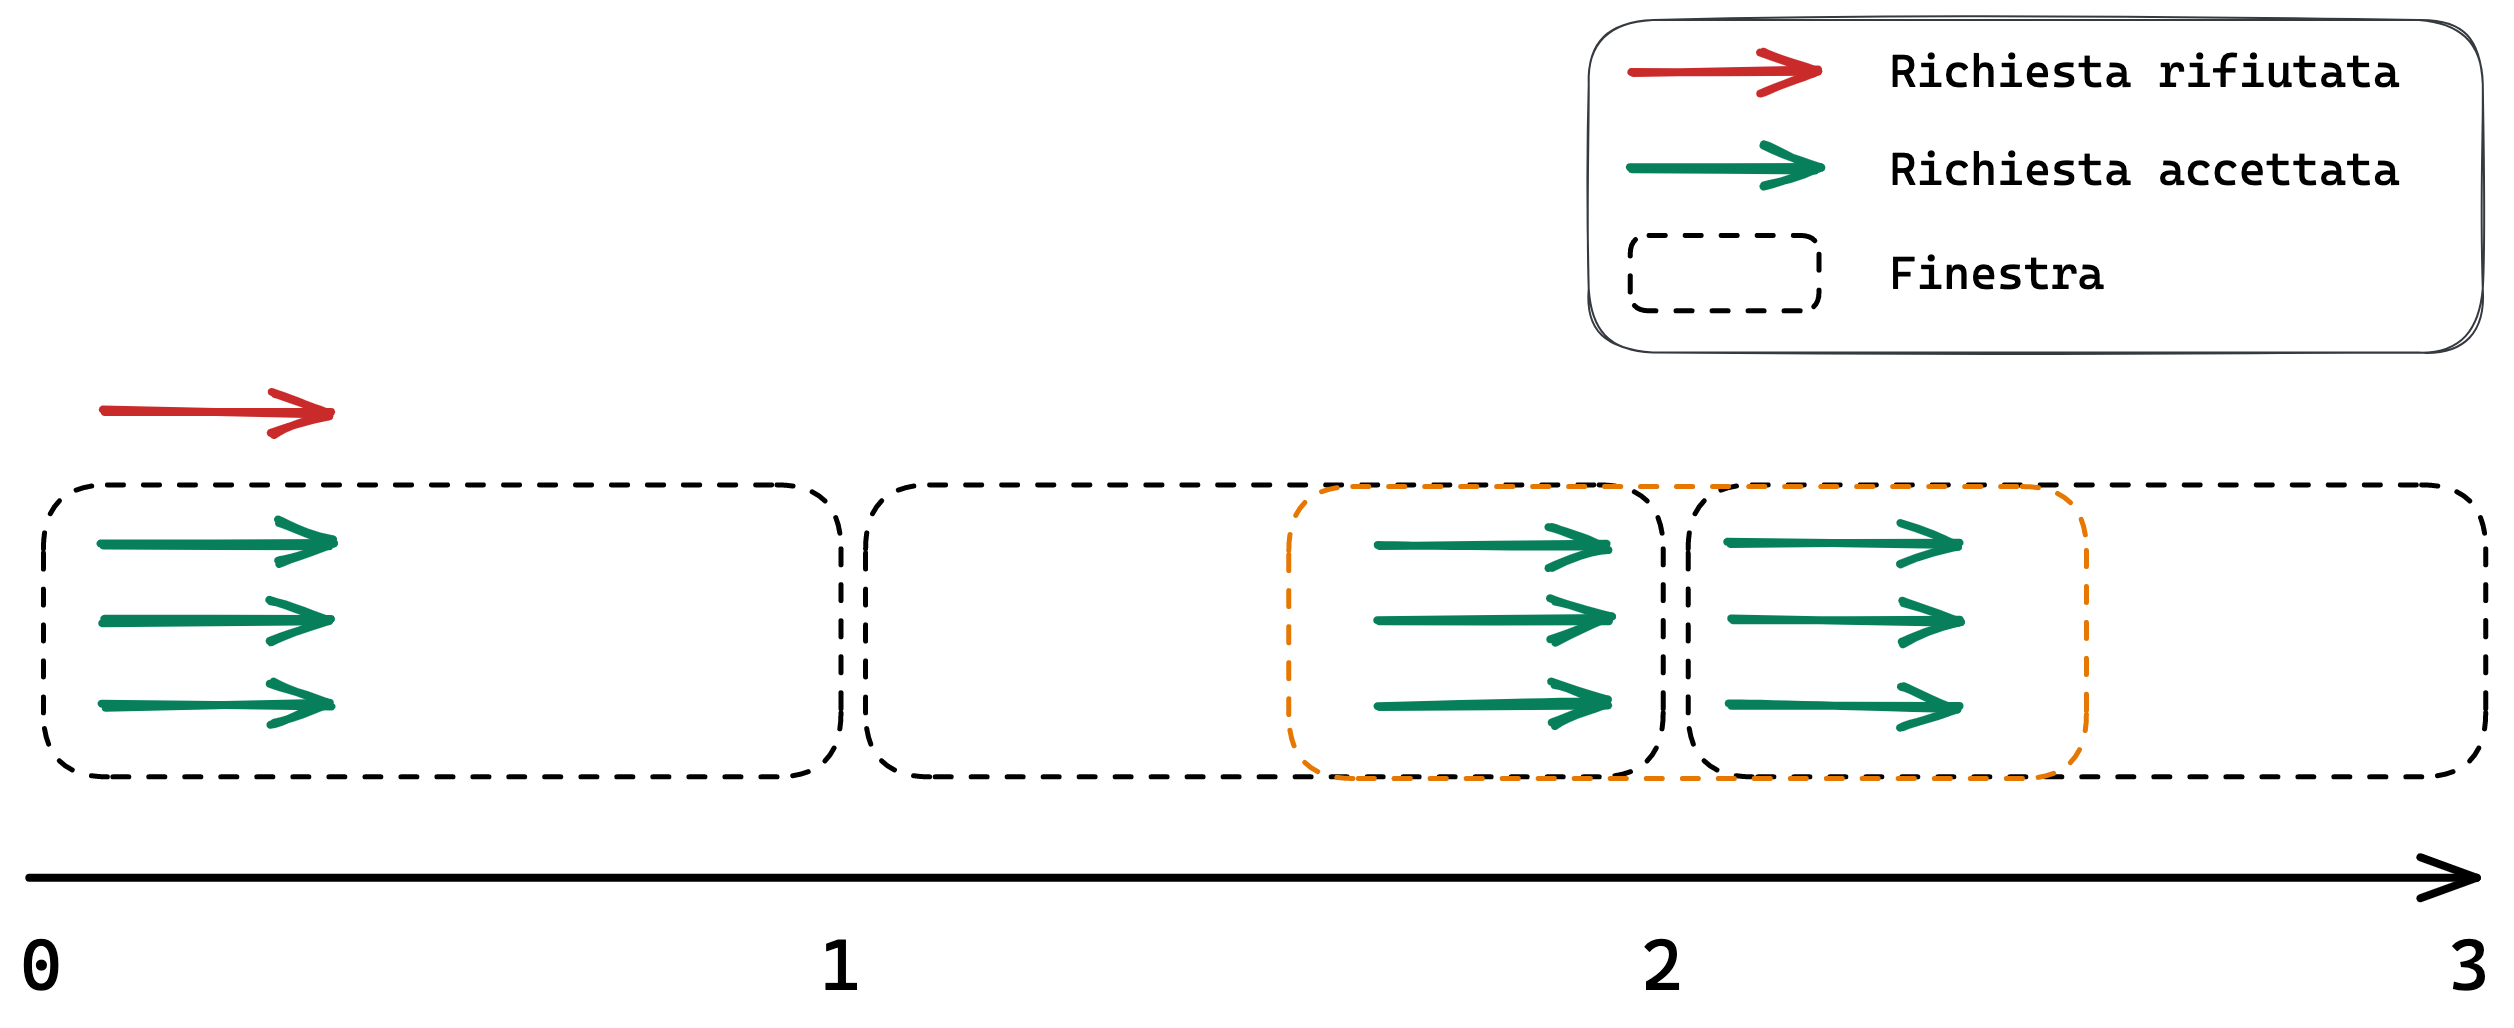
\includegraphics[width=12cm]{./immagini/mieimmagini/fixed_window.png}
        \label{fixed window diagram}
        \caption{diagramma Rate-limiting fixed window }
        \end{figure}
    
    \item \textbf{Token bucket :} Il funzionamento del token bucket prevede che non tutte le richieste di un servizio
    vengano mappate 1:1 con la richiesta di risorse, poiché alcune richieste potrebbero richiedere più risorse di altre.
    Per questo motivo, viene mantenuto un contatore di risorse, che viene scalato per ogni richiesta, del numero di
    token necessari per portare a termine il lavoro. Il contatore ha una frequenza di riempimento, ovvero a ogni unità
    di tempo viene reimpostato al suo valore massimo. Quando un utente o un'applicazione invia una richiesta al sistema,
    il sistema verifica se ci sono abbastanza token disponibili per soddisfare la richiesta. Se non ci sono abbastanza
    token, la richiesta viene respinta. In questo modo, le richieste vengono accettate solo se c'è abbastanza capacità
    per soddisfarle.
        \begin{figure}[H]
        \centering
        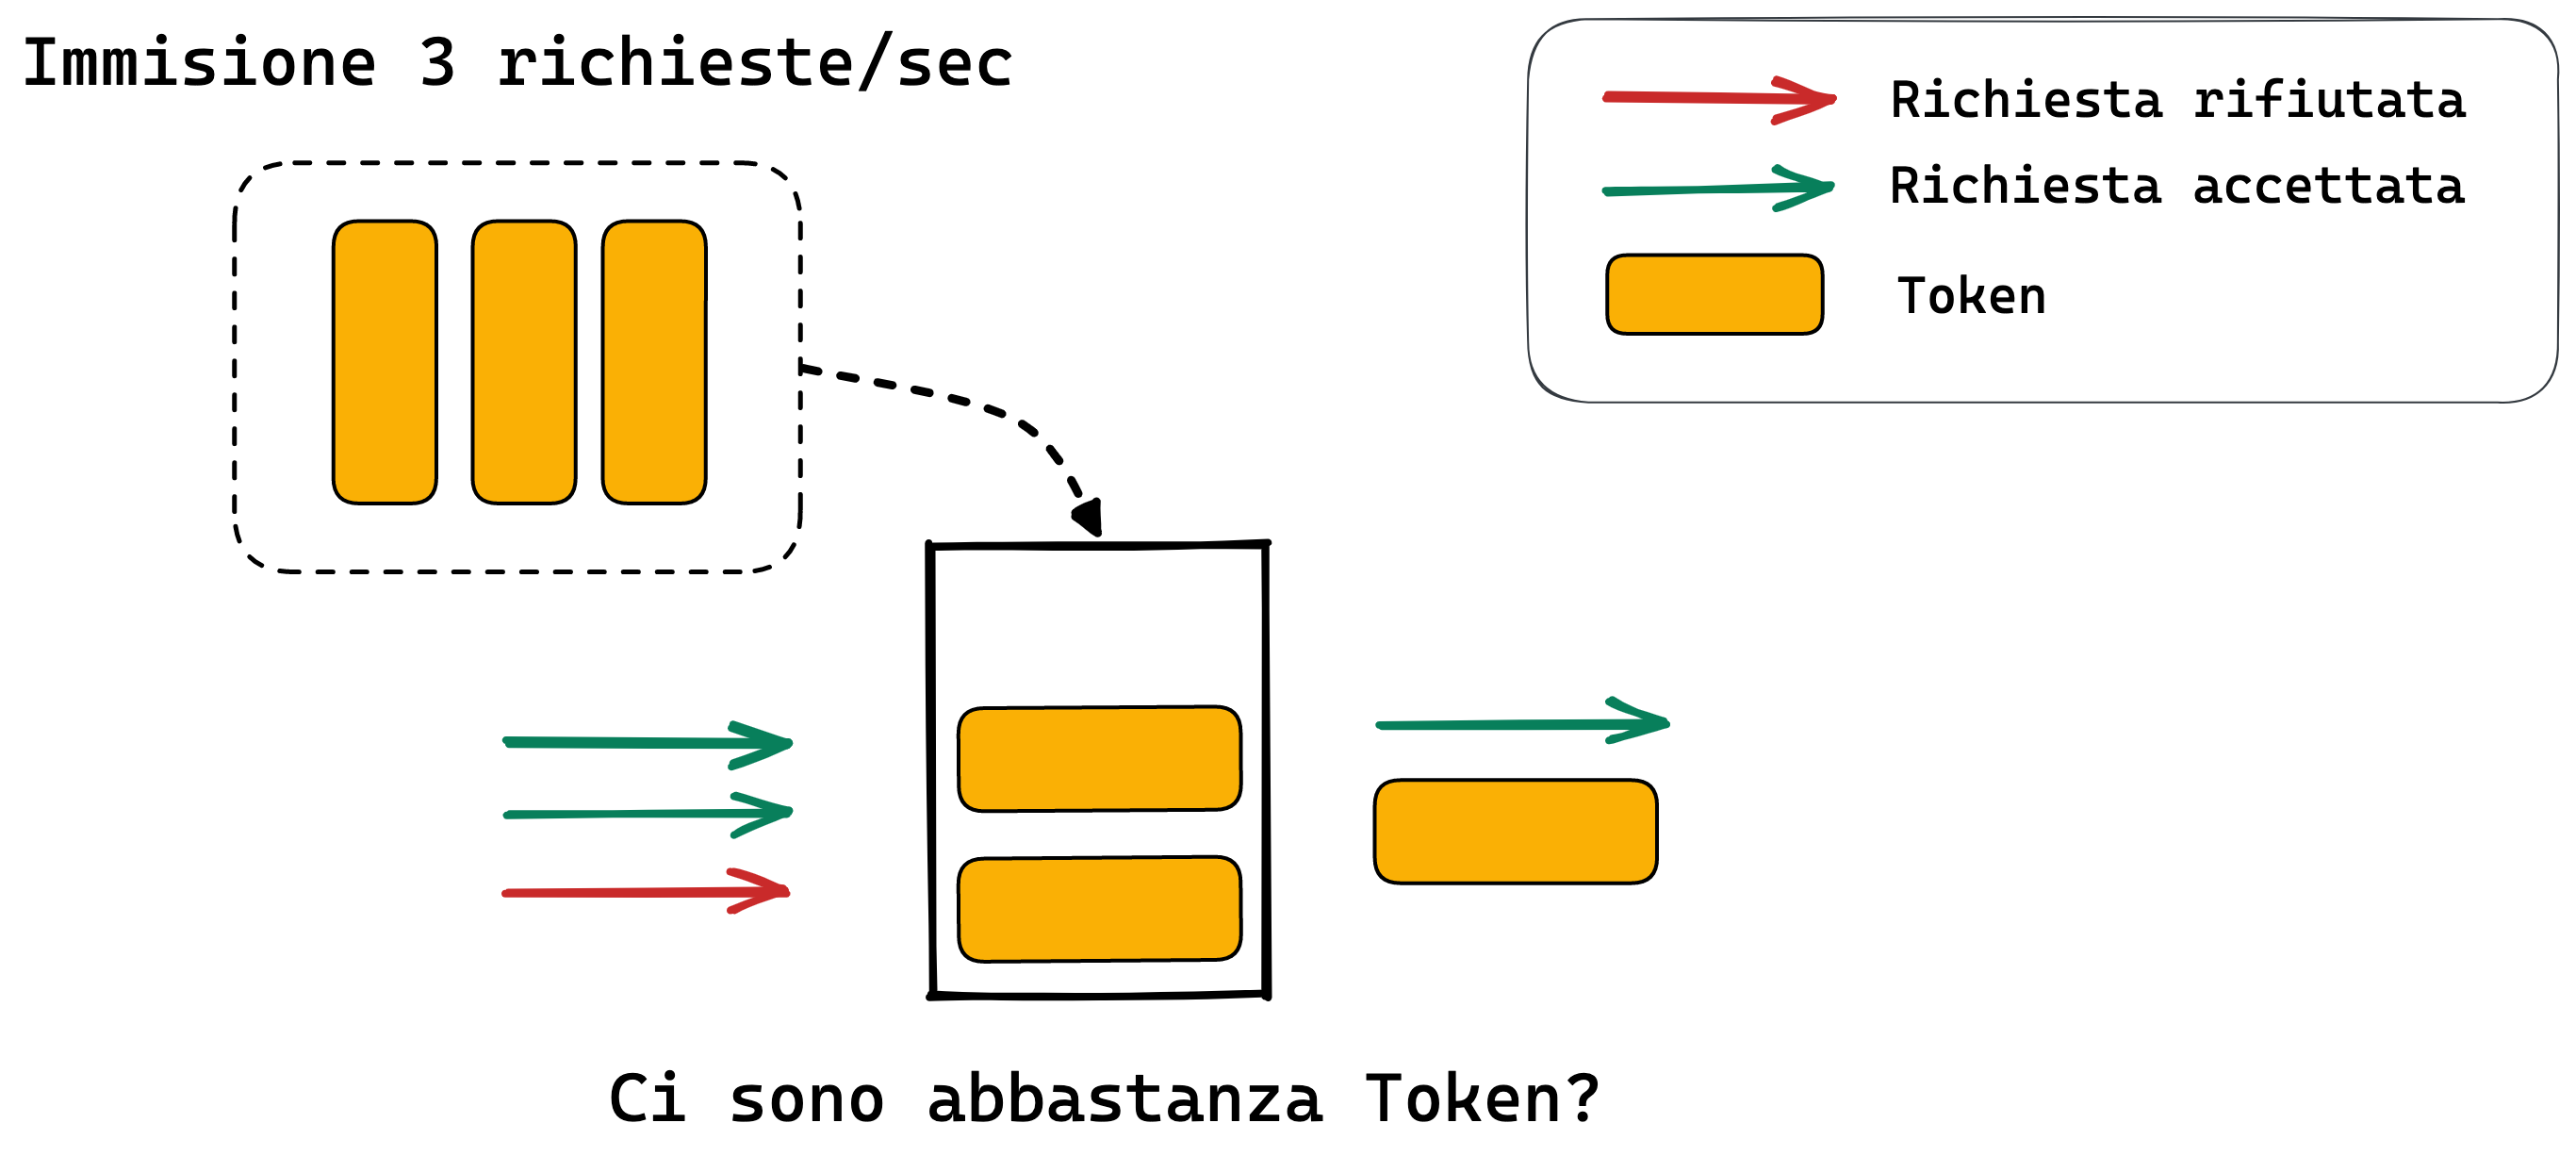
\includegraphics[width=12cm]{./immagini/mieimmagini/token_bucket.png}
        \label{token bucket diagram}
        \caption{diagramma Rate-limiting token bucket }
        \end{figure}
    
    \item \textbf{Leaky bucket :} L'idea di base è simile a quella del Token bucket ma invece di rispondere al numero di
    richieste liberando i token necessari fino a esaurimento, il tasso di elaborazione delle richieste viene regolato in
    modo uniforme. Questo significa che quando un pacchetto di dati arriva al sistema, se il secchio è già pieno, il
    pacchetto viene scartato. Nel mentre ad ogni unità di tempo viene elaborata una quantità di richieste corrispondente
    alla velocità di uscita del sistema. In questo modo, il flusso di dati in uscita non supera mai una certa soglia.
        \begin{figure}[H]
        \centering
        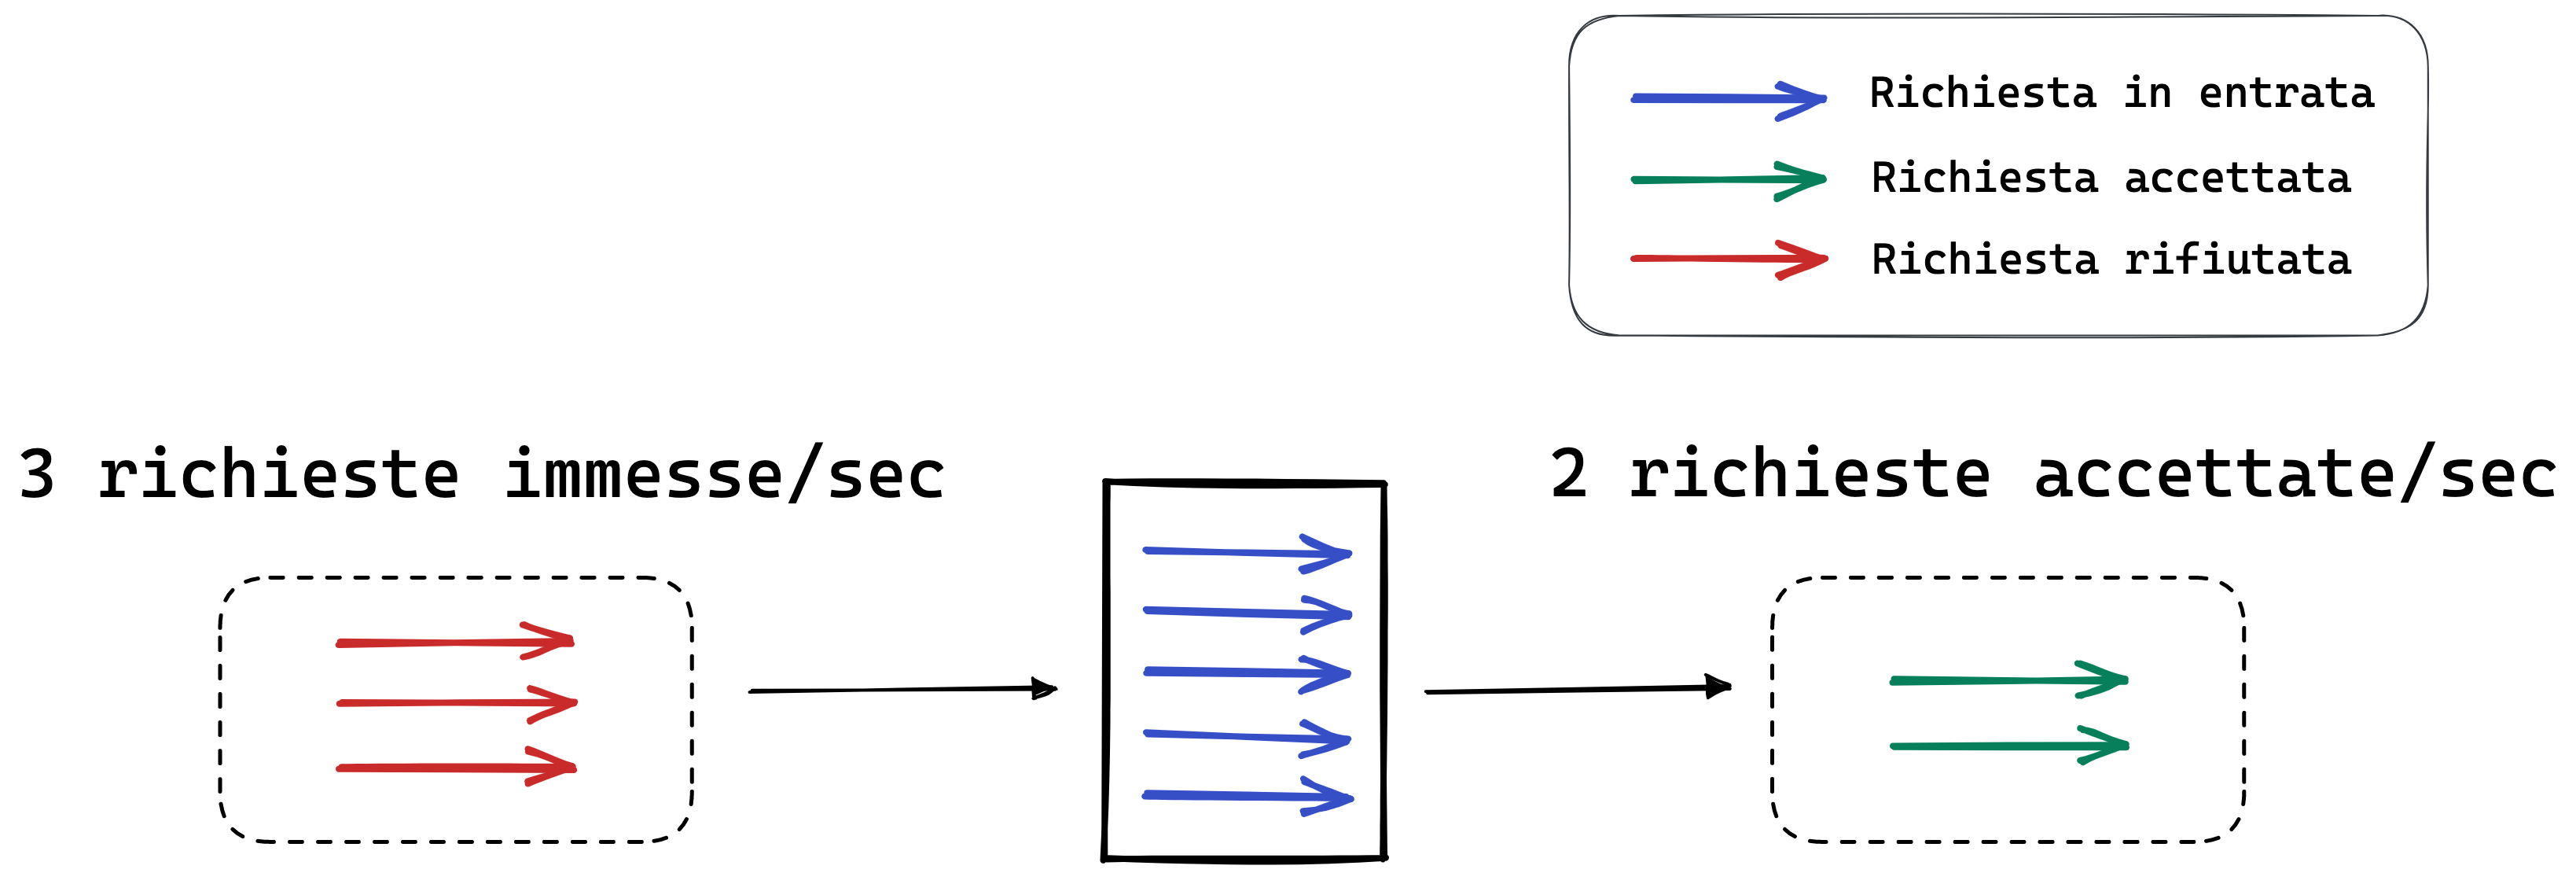
\includegraphics[width=12cm]{./immagini/mieimmagini/leaky_bucket.png}
        \label{leaky bucket diagram}
        \caption{diagramma Rate-limiting leaky bucket }
        \end{figure}
    
    \item \textbf{Sliding window:} La strategia di sliding window adotta un approccio simile alla Fixed Window, ma con
    una differenza fondamentale: esamina il tasso di richieste effettuate in un periodo di tempo continuo piuttosto che
    in intervalli fissi. Ad esempio, se il limite di richieste è fissato a 100 al minuto, la strategia prevede di
    controllare il numero di richieste effettuate nell'ultimo minuto e, nel caso superi il limite, rifiutare la
    richiesta. Questo approccio evita il potenziale sovraccarico del sistema alla fine di una finestra con un tempo
    prefissato, ma richiede la gestione di una finestra scorrevole, aumentando la complessità di
    implementazione.\begin{figure}[H]
        \centering
        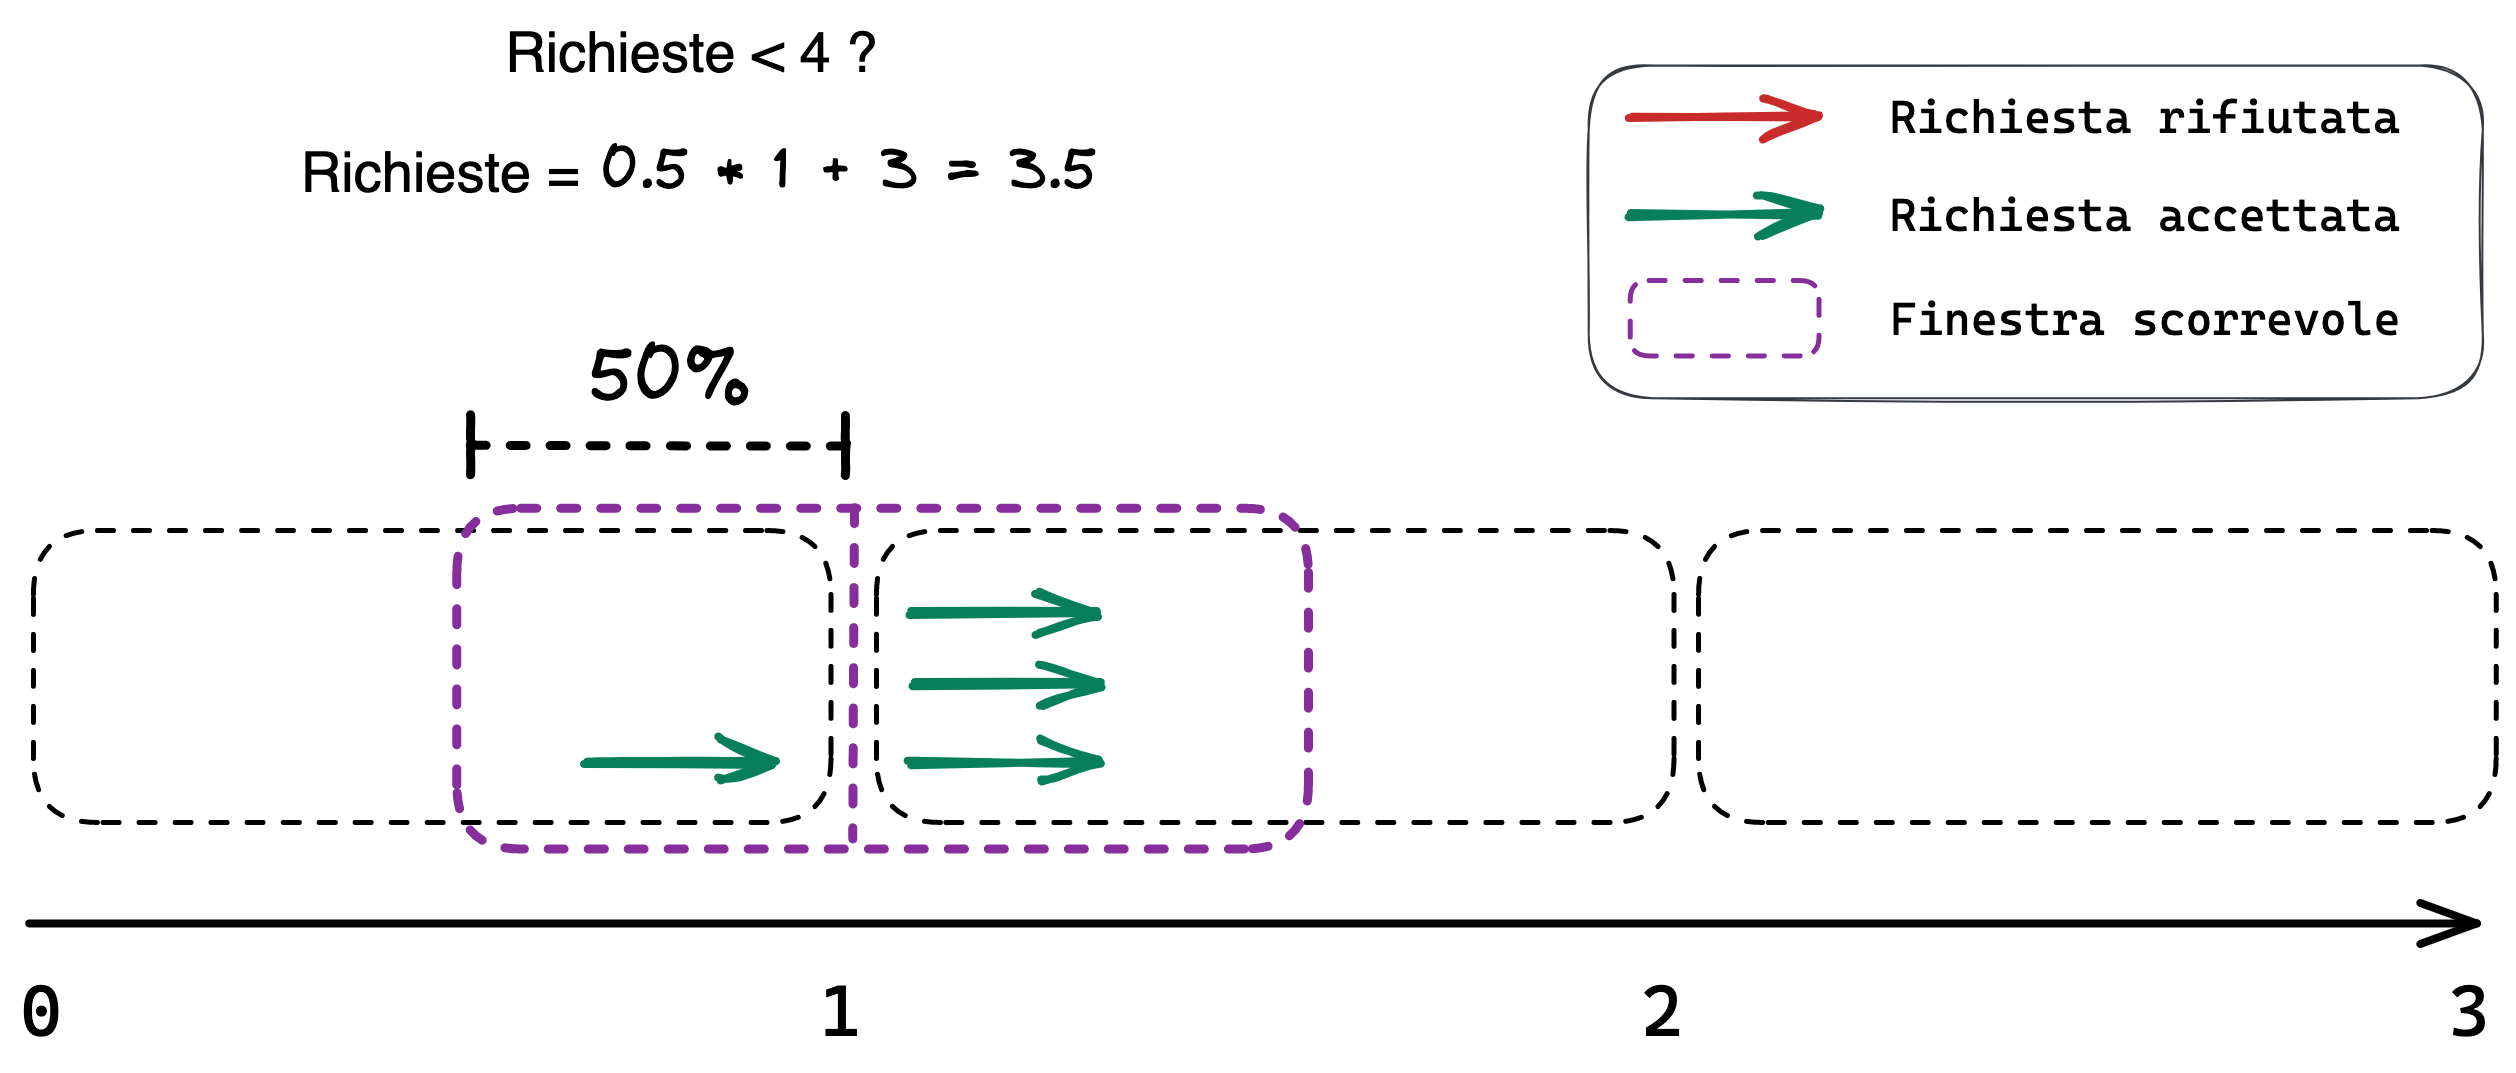
\includegraphics[width=12cm]{./immagini/mieimmagini/sliding_window.png}
        \label{sliding window diagram}
        \caption{diagramma Rate-limiting sliding window }
        \end{figure}
\end{itemize}
\clearpage

\section{zk-SNARK}
\label{sec:zk-SNARK}
L'acronimo zk-SNARK rappresenta l'espressione completa "Zero-Knowled Succinct Non-Interactive Argument of Knowledge".
Questa tecnologia è stata introdotta per la prima volta in un articolo scientifico pubblicato nel 2013 intitolato
"Pinocchio: Nearly Practical Verifiable Computation". Da allora, sono state apportate diverse migliorie alla tecnologia
e sono emerse numerose applicazioni in svariati settori. Le prime applicazioni significative di zk-SNARK sono state
implementate nel contesto della Blockchain, che rimane il settore dove la tecnologia è più conosciuta e applicata, per
fare alcuni esempi Etherium una delle Blockchain più accreditate  ha iniziato ad implementare la tecnologia nella sua
rete dal 2016, e il suo fondatore Vitalik Buterin ha scritto in un articolo sull’argomento: “Perhaps the most powerful
cryptographic technology to come out of the last decade is general-purpose succinct zero knowledge proofs, usually
called zk-SNARKs” (Forse la tecnologia crittografica più potente emersa nell'ultimo decennio è quella chiamata
zk-SNARK).

Zk-SNARK, come suggerisce il nome, rappresenta una tecnologia fondata sul protocollo crittografico zero-knowledge proof,
il quale consente a una parte (il dimostratore) di dimostrare a un'altra (il verificatore) la veridicità di
un'affermazione senza rivelare nessuna informazione ulteriore. Inoltre questo processo di dimostrazione, viene
effettuato in modo da ottenere una prova, in cui sia la dimensione della prova, che il tempo necessario per verificarla
crescono molto più lentamente rispetto al calcolo da verificare e senza la necessità di interazione bidirezionale tra le
due parti coinvolte.

Di seguito esamineremo meglio le singole parti che compongono la tecnologia zk-SNARK, analizzando i suoi componenti
chiave per ottenere una panoramica completa e concisa.

Prima di addentrarci nella descrizione delle componenti che utilizzeremo, è importante introdurre il campo di
applicazione dei teoremi e delle proprietà che andremo a utilizzare. In particolare, nei prossimi paragrafi lavoreremo
in un dominio di campi finiti, che è un dominio algebrico dove l'insieme dei numeri è finito e rispetta determinate
proprietà algebriche come l'addizione, la sottrazione, la moltiplicazione e la divisione. Per le loro proprietà i campi
finiti svolgono un importante ruolo in diversi algoritmi crittografici.

\subsection{Zero-Knowledge}
\label{sec:Zero-Knowledge}

Come accennato precedentemente, Zero-Knowledge proof è un protocollo crittografico in cui una parte dimostra di
conoscere una determinata informazione a un'altra parte, senza rivelare alcuna informazione aggiuntiva su di essa. Per
esempio, se Alice vuole dimostrare a Bob di conoscere la password del suo account, senza rivelargli la password stessa,
può utilizzare un protocollo di tipo Zero-Knowledge. In questo modo, Alice può dimostrare a Bob di sapere qual è la
password corretta senza rivelarla, proteggendo così la sua privacy e la sicurezza del suo account. Come è possibile
tutto questo? grazie a diverse tecniche crittografiche e tanta matematica.

Formalmente le prove di tipo Zero-Knowledge non sono dimostrazioni di carattere matematico, ma probabilistiche, il che
significa che c'è sempre una probabilità che un dimostratore scorretto riesca a dimostrare la veridicità di
un'affermazione a un verificatore onesto. Esistono tuttavia tecniche per ridurre questa probabilità a valori piccoli a
piacere.

% TODO CITARE "interactive proof systems"
Il primo articolo che definisce il costrutto è “The Knowledge Complexity of Interactive Proof-Systems"
\cite{10.1145/22145.22178} pubblicato nel 1985, dove  gli autori introducono il concetto di “Zero-Knowledge proof” come
un tipo di "interactive proof systems" (un modello computazionale che simula lo scabio di messagi tra due individui) in
cui il verificatore non apprende nulla oltre alla verità dell'affermazione che viene dimostrata.

Per poter costruire un sistema Zero-Knowledge proof per una particolare affermazione abbiamo bisogno che la prova
generata soddisfi le seguenti prorpietà :

\begin{itemize}
    \item \textbf{Completezza :} Se l'affermazione da dimostrare è vera, allora un verificatore onesto (cioè che segue
    correttamente le regole del protocollo) verrà convinto della veridicità da un dimostratore onesto.
    \item \textbf{Correttezza :} Se l'affermazione è falsa, nessun dimostatore disonesto può convincere un verificatore
    onesto che essa è vera, se non con una piccola probabilità.
    \item \textbf{Zero-knowledge :} Se l'affermazione è vera, nessun verificatore apprende altro se non il fatto che
    l'affermazione è vera.
\end{itemize}

Le tre proprietà appena viste descrivono Zero-Knowledge proof da un punto di vista formale ma per avere una visione più
intutiva del protocollo è utile vedere il flusso di funzionamento attraverso un esempio. L’esempio in questione è tratto
da un famoso articolo di Jean-Jacques Quisquater "How to Explain Zero-Knowledge Protocols to Your
Children” \cite{crypto-1989-1692} ne estrapolerò solo le parti esenziali alla tratazione, ma ne consiglio la lettura.

L’esempio riguarda una caverna a forma di anello, nella quale è posta a metà del percoso una porta che impedisce il
completamento del tragitto, a meno di non conoscere una parola segreta. Supponiamo l'esistenza di due parti, Peggy - che
conosce il segreto della porta e agirà da dimostratrice - e Victor - che invece non conosce il segreto e sarà il
verificatore. Peggy vuole dimostrare a Victor di sapere come superare la barriera senza però rivelare il segreto. Per
fare ciò, Peggy propone a Victor di seguire una strategia: dapprima stabiliscono un nome per identificare i due percorsi
(ad esempio, A e B), poi Victor rimane fuori dalla caverna mentre Peggy sceglie uno dei due percorsi. Dopo qualche
minuto, Victor entra nella caverna e chiama ad alta voce il nome di uno dei due percorsi, a quel punto Peggy dovrà
uscire dal percorso chiamato da Victor. Victor accetta la proposta, ma con una condizione: il processo dovrà essere
ripetuto più volte. Dopo diversi tentativi, Victor si convince che Peggy conosca effettivamente il segreto per superare
la barriera. Possiamo calcolare questa probabilità utilizzando la distribuzione binomiale, dove la probabilità di
successo \( p \) è del 50\% e il numero totale di prove \( n \) è 10. La probabilità di indovinare correttamente tutte le 10 scelte
di Victor è data dalla seguente formula: \[ P = p^n = 0,5^{10} = 0,0009765625 \]